\documentclass[12pt]{report}
\usepackage{apacite}
\usepackage[utf8]{inputenc}
\usepackage{graphicx}
\usepackage[romanian]{babel}
\usepackage[left=1in, right=1in, top=1in, bottom=1in]{geometry}
\setcounter{secnumdepth}{3}
\usepackage{mathptmx}
\usepackage[pagestyles]{titlesec}
\linespread{1.25}

\begin{document}

\begin{titlepage}
 
\newcommand{\HRule}{\rule{\linewidth}{0.5mm}} 
\center
\textsc{UNIVERSITATEA „BABEŞ-BOLYAI” \\
FACULTATEA DE MATEMATICǍ ŞI INFORMATICǍ \\
SPECIALIZAREA INFORMATICǍ}\\[5cm]
\textsc{\large Lucrare de diplomă}\\[0.5cm]

\HRule \\[0.4cm]
{\LARGE  \bfseries STUDIUL EFICIENȚEI FOLOSIRII UNEI ARHITECTURI BAZATE PE MICROSERVICII ÎNTR-UN SISTEM DE PLATĂ A UTILITĂȚILOR}\\[0.4cm]
\HRule \\[1.5cm]
 
\begin{minipage}{0.4\textwidth}
\begin{flushleft} \large
\emph{Coordonatori științifici:}\\
lect. dr. \textbf{Mircea Ioan Gabriel }
\end{flushleft}
\end{minipage}
~
\begin{minipage}{0.4\textwidth}
\begin{flushright} \large
\emph{Absolvent:} \\
\textbf{Petruțiu Paul-Gabriel} 
\end{flushright}
\end{minipage}\\[6cm]
 
{\large \textbf{Cluj-Napoca}}\\[2mm]
{\large \textbf{2019}}
\vfill
\end{titlepage}

\tableofcontents
\cleardoublepage
\listoffigures

\chapter{Introducere} 

\chapter{Concepte de bază} 
  \section{Arhitectura unei aplicații soft}
  	\paragraph{}
  	Deoarece tot mai multe companii din diferite domenii au nevoie de o aplicație software personală pentru a-și imbunatații calitatea produselor, pentru prezentarea produselor sau pentru ușurarea unor activități din cadrul companiei, cererea de a crea cod este tot mai mare. Pentru ca aplicațiile sa fie usor de dezvoltat, pentru ca o imbunătățire sa poată fi implementată fără prea mult efort, este important ca aplicația sa aibă la baza o structură bine definită. Acest lucru face ca o aplicație să fie ușor de intreținut în decursul timpului.
  	\paragraph{}Având in vedere standardul IEEE Std 1471, arhitectura unei aplicații soft este definită ca „Organizarea fundamentală a unui sistem încorporat în componentele sale, relațiile dintre ele și mediul, precum și principiile care conduc proiectarea și evoluția sa.”(\cite{hilliard2000ieee})
  	\paragraph{}Așadar, putem considera un sistem ca fiind o aplicație sau un set de aplicații care impreună rezolvă diferite probleme.
  \section{Șabloane de proiectare}
  \paragraph{}Un șablon de proiectare este reprezentat ca fiind o solutie cunoscuta pentru o problema recurenta.
    \paragraph{}„Șabloanele de proiectare pot fi văzute ca un mijloc de a reuși reutilizarea pe scară largă prin captarea unei practici de design de dezvoltare a software-ului de succes într-un anumit context” (\cite{alencar1996formal}).
  Deci, un șablon de proiectare reprezintă doar în mod abstract o soluție pentru o problemă. Din acest motiv, șabloanele de proiectare pot fi aplicate în oricare limbaj de programare, in funcție de contextul problemei.
  \paragraph{}Motivul pentru care șabloanele de proiectare sunt relevante indiferent de limbajul de programare folosit, este acela că șabloanele de proiectare sunt doar concepte despre cum ar trebui să fie impementat codul si nu cod propriu zis.
  \section{Serviciu Software}
  \paragraph{}
  Un serviciu este o componentă a unei aplicații soft care furnizează una sau mai multe funcționalități altor componente din sistem. Aceste componente pot să fie aplicații web, mobile sau chiar alte servicii.
  \paragraph{}
  Spre exemplu, putem presupune ca avem un site în care utilizatorii pot să achite fucturile de curent, gaz, etc.. În momentul în care utilizatorul efectuează o plată, browser-ul va apela un serviciu care va procesa, în spate, aceasta tranzactie(verificarea daca suma introdusă este validă, dacă suma este disponibilă, etc.)
  \paragraph{}
  Sistemele ce folosesc mai multe servicii, similar cu exemplul expus mai sus, sunt considereate ca fiind sisteme care au la bază o arhitectură orientată pe servicii.
  \chapter{Aplicații Monolit}
  	\section{Ce este o aplicație monolit?}
  	\paragraph{}O aplicație monolit este o aplicație a cărei cod este scris in cadrul unei singure unitați structurale. Componentele din care este alcătuită aplicația sunt gândite in așa fel incât sa funcționeze împreună și să se folosească de acelasi spatiu de memorie si de aceleași resurse.
  	\paragraph{}Aplicațiile monolit sunt printre cele mai raspândite din lume. Acest fapt se datorează felului în care oamenii abordeaza problemele. O soluție de tip monolit este prima solutie pe care un programator o va avea, deoarece este un mod natural de a gandi. În plus, pentru multe din aplicații, o solutie monolit va fi soluția perfectă, având în vedere că multe companii mici spre medii doresc sa aiba o aplicație care să automatizeze anumite procese, procese care nu au o complexitate extrem de mare, iar numărul utilizatorilor nu este enorm. 
  	\paragraph{}Spre exemplu, să spunem că o firmă are un sediu destul de mare care are 5 săli de conferintă, având in vedere numărul mare de întâlniri din interiorul firmei, aceștia doresc o aplicație în care să poată rezerva o sala de conferintă pentru o anumită perioadă intr-o anumită zi. O astfel de aplicatie se poate realiza usor si rapid, sub forma unei aplicații web de tip server client(\ref{monolithicArhitecture}).
  	\begin{figure}[h]
  	\centering
  	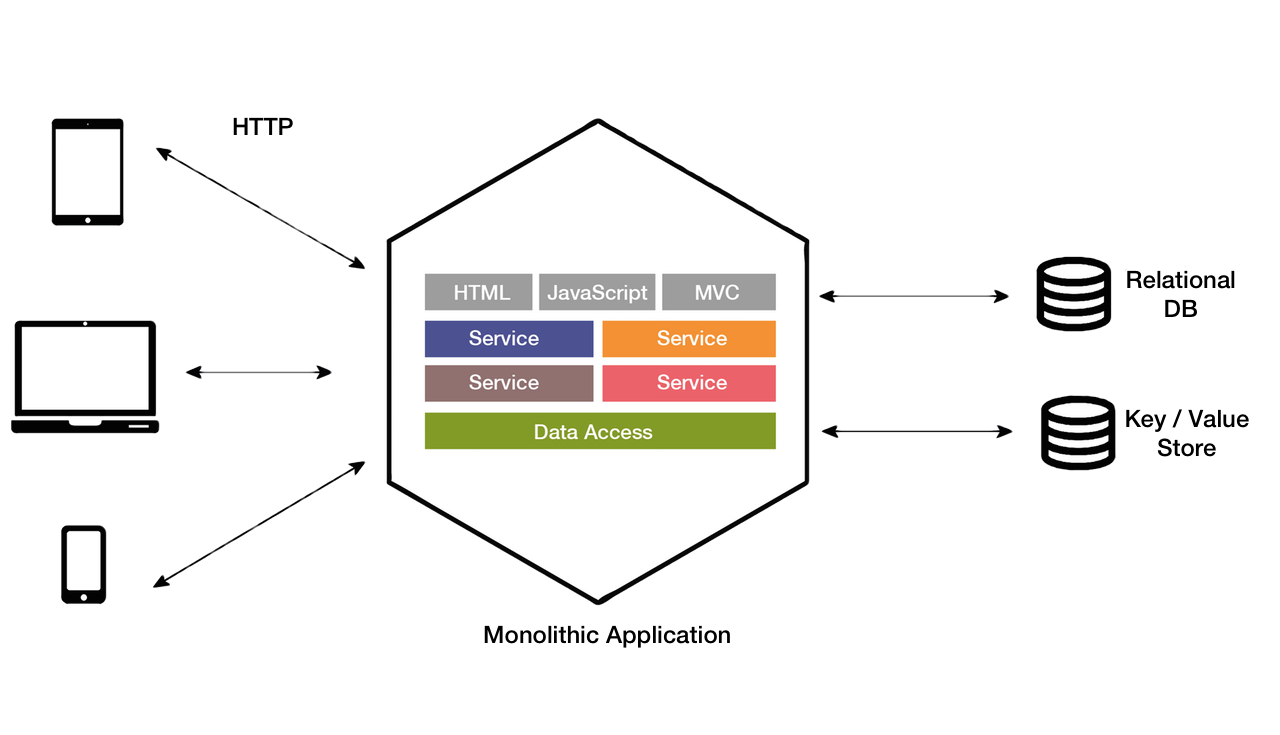
\includegraphics[scale=.2]{monolitFigure}
	\caption{Arhitectură Aplicație Monolit(imagine : http://bits.citrusbyte.com)}  
	\label{monolithicArhitecture}
  	\end{figure}
  	\section{Avantaje și dezavantaje}
  	\paragraph{}O aplicație monolit are mai multe avantaje in contextul unui business mic:
  	
  	\begin{itemize}
  	\item Faza de dezvoltare durează mai puțin timp, IDE-urile moderne reușind să genereze mult cod automat, ceea ce implică scădearea costurilor de producție.
  	\item Aplicația este usor de testat, automatizând procesul de testare a codului folosind o combinație de unit tests și integration test. 
  	\item Procesul de lansare în producție a unei aplicatii nu este complicat, deoarece este nevoie de rularea unei singure aplicații per server.
  	\end{itemize}
  	\paragraph{}Pe de altă parte, in momentul în care aplicația va creste ca și volum al codului, un număr mai mare de programatori vor trebui implicați în procesul de dezvoltare al aplicației, acest lucru nu este un lucru rău, doar ca aceștia vor intampina anumite impedimente:
  	\begin{itemize}
  	\item Cuplajul dintre componentele aplicației creste, iar acest fapt va îngreuna procesul de dezvoltare a unor noi functionalități, acest lucru va afecta timpul si costul necesar dezvoltării noii funcționalități.  
	\item Alegerea tehnologiilor folosite pentru dezvoltarea aplicației este permanentă.
	\item Integrarea/Intrarea unui programator in proiect va fi mai dificilă. Volumul aplicației fiind mare, va fi necesar un timp mai mare pentru înțelegerea tuturor funcționalităților si a decizilor luate pe proiect in trecut.
  	\end{itemize}
  	\paragraph{}Acestea sunt doar câteva dintre avantajele si dezavantajele unei aplicații monolit, dar sunt suficiente incât putem sublinia o idee generală. Aplicațiile bazate pe o arhitectura monolit sunt mai ușor de implementat în primă fază cu un cost mai redus, dar în momentul în care aplicația ajunge la un nivel mai avansat, este nevoie de o reconstruire parțiala sau totală a aplicației sau cel puțin este nevoie de o refactorizare care sa diminueze dezavantajele create de stilul arhitectural folosit. Majoritatea aplicațiilor încep ca și aplicații tip monolit, iar mai târziu se pot transaforma in aplicații cu arhitecturi bazate pe microservicii de exemplu.(\cite{thones2015microservices})
  \chapter{Arhitectura bazată pe servicii}
  	\section{Fundamentele arhitecturii bazate pe servicii}
  	\paragraph{}Unul din factorii care au dus la modificarea conceptelor despre cum trebuie să fie structurată o aplicație, a fost evolutia tehnologică rapidă și numărul tot mai ridicat de persoane care aveau acces la internet.
	\paragraph{}Arhitectura bazată pe servicii (în engleză „Servici Oriented Architecture”, prescurtat „SOA”), este un tip de arhitectură care s-a născut datorită nevoii tot mai mari de dezvoltare rapidă a cât mai multor funcționalități într-un timp cât mai scurt, si in paralel pe cât posibil.
	\paragraph{}Unul din motivele principale pentru apariția acestui stil arhitectural s-a datorat dorinție producătorilor ca o aplicație să poată sa fie folosită de pe diferite platforme. Dacă pentru fiecare platforma diferită era nevoie ca toată aplicația să fie rescrisă, costul ar fi fost prea mare, această soluție nu era plauzibilă. Datorită acestui fapt s-a decis că logica aplicației ar trebui să fie decuplată de partea din față a aplicației. În felul acesta, fiind necesară doar rescrierea  unei parți mult mai mici din aplicație pentru ca aceasta să poată functiona pe diferite tipuri de platforme. Odată cu această decizie, un nou stil arhitectural a apărut.
	\paragraph{}Pentru început, s-a incercat enunțarea a 8 principii, care ar trebui respectate intr-o arhitectură bazată pe servicii.
	\paragraph{}Acestea sunt:
	\begin{itemize}
	\item Serviciile sunt autonome.
	\item Serviciile sunt slab cuplate
	\item Serviciile trebuie să abstractizeaze logica pe care o folosesc.
	\item Serviciile împart un contract formal.
	\item Serviciile sunt compozabile
	\item Serviciile sunt refolosibile
	\item Serviciile nu au stare
	\item Serviciile se pot descoperii
	\end{itemize}
	\paragraph{}Din aceste 8 principii, primele 4 sunt cele mai importate, acestea reprezentând fundația arhitecturii bazate pe servicii. Toate cele 8 principii se suțin intre ele, dar primele 4 principii induc și restul.
  	\section{Principiile arhitecturii bazate pe servicii}
  	\subsection{Autonomia}
  	\paragraph{}Orietarea către servicii cere o atitudine serioasă atunci cand vine vorba de împărtirea lor in blocuri logice de sine stătătoare. Pentru ca serviciile sa fie fiabile și previzibile, trebuie sa se exercite un grad mai ridicat de control asupra resurselor pe care ele le folosesc.
  	\paragraph{}Odată cu cresterea nivelului de control al unui serviciu asupra propriului context de executie, se reduc dependințele din serviciu, ceea ce ne duce spre un alt principiu, cel al cuplajului slab. Chiar dacă exclusivitatea asupra logicii pe care un serviciu o encapsulează nu poate să fie deplină, principalul obiectiv este atribuirea unui nivel rezonabil de control asupra oricărei logici pe care o prezintă intr-un moment al executiei.
  	\paragraph{}Având in vedere că pot exista deferite metode de a masura autonomia, este bine facem distincție intre ele. Spre exemplu, un serviciu poate avea mai multe nivele de autonomie:
    \begin{itemize}
    \item Autonomie la nivelul serviciului. În acest tip de autonomie granițele dintre servicii sunt bine definite, dar resursele folosite de server pot să fie distribuite cu alte servicii. Spre exemplu, putem avea un serviciu care encapsulează un mediu de lucru mai vechi, acesta deja fiind folosit de un alt serviciu vechi.
    \item Autonomie pură. Când vorbim de autonomie pură, ne referim la faptul ca intreaga logică de care se folosește un serviciu, îi serveste exclusiv lui. 
    \end{itemize}
    \paragraph{}Cu siguranță, se dorește ca un număr cât mai mare sa fie de servicii pur autonome, deoarece acestea ar rezolva usor problemele de concurență și ar impinge serviciile importiva problemei „unui singur punct de eșec” (în engleză „single point of failure”). Oricum, pentru a se atinge această performanță, procesul de dezvoltare este mai lung, deoarece logica din servcii trebuie să fie rescrisă, iar partea de lansare în execuție a serviciului ar avea nevoie de atenție sporită. Așadar efortul si costurile ar crește, iar uneori aceste sacrificii nu sunt posibile.
  	\subsection{Cuplajul slab}
  	\paragraph{}Nimeni nu poate să prezică în direcție va evolua domeniul IT. Nu se poate știi evoluția pentru automatizarea soluților, integrarea sau schimbarea lor, acestea fiind influențate de cauze din afara mediului IT. Având in vedere faptul ca în cazul unei modificăre neprevazută programatorii trebuie să fie gata să răspundă într-o manieră eficientă, un lucru necesar este lucrul cu forme abstracte ale serviciilor si mesajelor. Acest fapt, susține agilitatea de a compune o soluție folosind serviciile disponibile.
  	\paragraph{}Putem spune că cuplajul între doua unități logice și structurale poate fi văzut ca o măsurătoare a dependințelor dintre ele. Ceea ce înseamnă ca un număr mare de dependințe poate fi definit ca și un cuplaj mare. În cazul în care nu exista dependințe între două servicii, putem spune ca ele sunt decuplate. Prin implementarea consisteantă a cuplajului slab, unitățile logice dezvoltate ulterior dobândesc independență. Din acest fapt, în timp, se acumulează o multitudine de servicii care sunt blocuri logice de sine statatoare, care pot fi folosite in noi compoziții, și care pot fi întreținute ușor, fără a influența alte servicii.
  	\subsection{Abstractizarea}
  	\paragraph{}Abstractizarea este un concept cunoscut in programare, fiind unul din principiile fundamentale ale paradigmei programarii orietate pe obiecte. Cam în aceeași directie se indreaptă si abstractizarea logicii din servicii. Acest concept sugerează că un serviciu ar trebui scris ca o cutie neagra, adică ascunzând detaliile de un potențial consumator. Acest lucru se realizează folosind contracte pentru fiecare serviciu, acesta limitând accesul catre serviciu. Cu ajutorul unui contract, se obține foarte ușor un grad mare de separare între ce este privat si ce este public pentru consumator. Ca rezultat, acest concept susține conceptul dezbătut anterior, cel al cuplajului slab.
  	\paragraph{}Dacă ar fi să discutăm despre cantitatea de logică pe care un serviciu o poate expune, putem spune ca nu există nici o limitare din acest punct de vedere. Un serviciu poate fi creat cu scopul de a servii îndeplinirii unui singur feature sau poate fi un punct de intrare în întreaga aplicație.
  	\paragraph{}Așadar se poate observa că întreaga atenție se poate îndrepta se modul in care un contract este conceput. Cu cât mai multă informație este expusa prin contract, cu atat mai puțină informație poate fi abstractizată. Cu cât un contract este mai generic, cu atat mai mult crește capacitatea lui de a fi reutilizat.
  	\subsection{Contractul Formal}
  	\paragraph{}În mod normal, serviciile trebuie definite in mod formal folosind unul sau mai multe documente descriptive. Spre exemplu, pentru un serviciu web se folosesc documente de tip WSDL și o schema XSD. Documentele care ajuta la descrierea unui serviciu pot fi considerate colectiv ca fiind un contract de servicii. Conform arhitecturii bazate pe servicii, un contract al unui serviciu ar trebui sa definească urmatoarele lucruri:
  	\begin{itemize}
  	\item Punctele de acces in serviciu (în engleză „endpoint”).
  	\item Fiecare operație pe care o poate efectua serviciul.
  	\item Pentru fiecare operație, formatul datelor de intrare cât și al celor de ieșire
  	\item Regulile si caracteristicile serviciului.
  	\end{itemize}
  	\paragraph{}Definirea contractelor necesită o atenție sporită pentru ca acestea sunt distribuite printre servicii. După momentul in care sunt lansate in execuție, definiția contractelor s-ar putea să devină o dependința pentru o sursa externă, ceea ce înseamnă că trebuie avut grijă ca definițiile din contract să nu sufere schimbări după lansarea principală. Prin urmare, contractele formale reprezintă un principiu de baza intr-o arhitectura bazată pe servicii. În plus acest concept susține alte principii despre care am discutat, aceastea fiind: abstractizarea și cuplajul slab, dar și alte principii care nu au fost abordate in detaliu precum: compozabilitatea si descoperirea serviciilor.
\chapter{Arhitectura bazată pe microservicii}
	\section{Ce sunt microserviciile}
	\paragraph{}Microserviciile sunt un concept apărut nu cu mult timp in urmă, iar acesta este unul dintre motivele pentru care aceastea nu au o definiție exactă. Un alt motiv ar putea fi acela că microserviciile sunt o derivare ușoară a serviciilor. Având in vedere încercările de a crea o definiție pentru microservicii, putem găsii cateva caracteristici comune. Una dintre aceste definiții sugerează ca arhitectura bazată pe microservicii este, de fapt o arhitectură bazată pe servicii în care toate principiile au fost aplicate corect.
	\paragraph{}Dacă ar fi să extragem aceste caracteristici speciale pe care trebuie sa le aibă un microserviciu, putem pornii chiar de la cuvantul „microserviciu” care ar putea fi imparțit in „micro” si „serviciu”. Deci microserviciile sunt de fapt servicii de dimensiune mică, autonome si fara stare, acestea lucrând impreună. 
	\paragraph{}Daca tot ne bazăm pe „definițiile” din mediul online, putem găsi și mici diferențe intre arhitectura bazată pe servicii si cea bazată pe microservicii. Spre exemplu comunicarea in servicii se face in general cu ajutorul unui service bus, iar in microservicii se incearcă folosirea unor sisteme de mesaje mult mai simple, serviciile sunt contruite printr-o abordare „distribuie cât mai mult” iar microserviciile printr-o abordarare „distribuie cat mai puțin”. Serviciile se orientează mult mai mult pe reutilizare, în schimb microserviciile sunt orientate in primul rând pe un cuplaj cat mai mic, sau inexistent, acest lucru susținând principiul cuplajului slab.
	\section{Comunicarea între microservicii}
		\subsection{Diferite tipuri de comunicare}
	\paragraph{}Dacă vrem să discutăm despre comunicarea intre microservicii, comunicarea ar putea să fie sincronă sau asincronă. În cazul microserviciilor se preferă comunicarea asincronă. Chiar daca comunicarea sincronă este mai ușor de implementat, spre exemplu, se face un call catre un microserviciu și se asteaptă pana când acesta returnează un mesaj sau pana eșuează. Dar acest lucru înseamnă că cele două servicii sunt acum cuplate, acest lucru fiind împotriva unui principiu de bază, cel al cuplajului slab. Daca vorbim despre comunicare asincronă, ne referim la faptul că un call este creat, dar restul execuției nu este blocată până se primește un raspuns, acest lucru fiind favorabil atunci când logica din spate durează mai mult timp. Spre exemplu, dacă dacă se efectuază un call care ar trebui să aducă o listă mai mare de obiecte pentru a fi afișate. Nu se doreste ca interfața pe care utilizatorul o vede să fie blocată, așadar comunicarea asincronă va permite asta.
	\paragraph{}Comunicarea între microservicii se poate realiza sub forma de call-uri, așa cum deja am precizat mai sus, dar nu este singura variantă. O alta modalitate de comunicare între microservicii este comunicarea bazată pe evenimente, care funcționează invers intr-o oarecare masură. Acest lucru înseamnă că in momentul in care se produce o acțiune într-un microserviciu, aceasta produce un eveniment prin care anunță alte microservicii sau alte unități ale aplicației că o modificare a fost efectuată, iar acestea, având o logică implementată, vor putea gestiona situația.
		\subsection{Utilizarea unui broker de mesaje}
	\paragraph{}Un broker de mesaje reprezintă de fapt o componentă exterioară a aplicației, care are scopul de stoca si persista mesajele sau evenimentele până cand acestea sunt consumate de serviciul necesar. Un broker de mesaje necesar atunci cand vorbim de o comunicare asincronă, mai ales cand este vorba de comunicare cu ajutorul evenimentelor.
	\paragraph{}Un exemplu care determină utilitatea unui broker de mesaje, ar putea fi următorul. Să presupunem ca avem un magazin online, si avem un microserviciu care se ocupă de plasarea unei comenzi, iar un microserviciu se ocupă cu logica pentru transportul pachetului. Dacă am presupune că microserviciul pentru transport nu funcționează, printr-o metodă sincronă de comunicare, rezultatul ar fi aruncarea unei exceptii care mentionează ca nu se poate plasa o comandă. Dacă se foloseste un broker de mesaje, comanda va fi procesată cu succes iar in momentul in care microserviciul care se ocupă de transportul produsului va functiona, procesul de livrare al produsului va începe.
	\section{Avantaje și dezavantaje ale microserviciilor}
	\paragraph{}Ca să vorbim de avantaje și dezavantaje, ar trebui să realizăm o comparație, iar pentru aceasta comparație ne vom folosii de o arhitectură monolit. Așadar in figura de mai jos (\ref{movsmicr}) putem vedea diferentele de structură. 
	\begin{figure}[h]
  	\centering
  	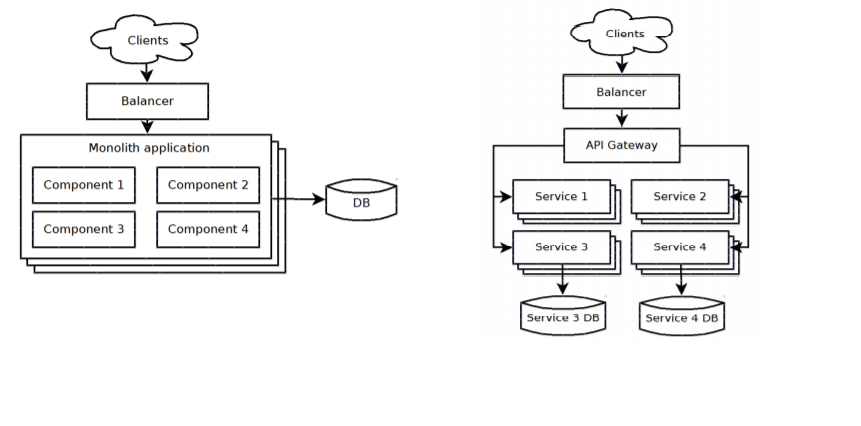
\includegraphics[scale=1]{movsmicr}
	\caption{Arhitectură monolit vs arhitectură bazată pe microservicii}\cite{savchenko2015microservices}  
	\label{movsmicr}
  	\end{figure}
  	\subsection{Avantaje}
  	\paragraph{}Un avantaj al microserviciilor este oferit chiar de structura lor, dupa cum se obesrvă si in figura \ref{movsmicr}, microserviciile sunt independente unele de celelalte, acest lucru făcând mult mai ușoară dezvoltarea și îmbunătățirea lor. Mult mai rapidă intelegerea codului iar prin urmare, in oposiție cu o aplicație monolit, integrarea unui om nou pe proiect este mai usoară.
  	\paragraph{}Microserviciile pot să fie văzute ca niste bucăți de lego care împreună crează o intreagă aplicație. Din acest motiv microserviciile sunt usor scalabile. Iar cand ne referim la scalabilitatea microserviciilor, ne referim la o scalabilitate pe orizontală. Având in vedere dimensiunea unui microserviciu în comparație cu dimensiunea intregii aplicații, e foarte evident că un microserviciu poate gestiona mult mai usor si mai flexibil resursele unui server. Acest lucru înseamnă că resursele unui server mai putin folosit, pot fi redistribuite pentru un server mai ocupat, pentru a se evita blocajele \cite{singleton2016economics}. Așadar, din cauza flixibilitații și a capacitații de scalare pe orizontală, un sistem bazat pe microservicii are un cost mai mic decăt un sistem monolit, deoarece nu toate microserviciile trebuie scalate in aceeași masură, iar o aplicație monolit nu iti poate oferii optiunea de a alege. \cite{newman2015building}
  	\subsection{Dezavantaje}
  	\paragraph{}Chiar dacă structura acestei arhitecturi aduce avantaje, aceasta aduce si dezavantaje. De exemplu, datorită complexității pe care o are o arhitectură bazată pe microservicii, o aplicație mica sau medie, ar avea doar de pierdut, timpul de dezvoltare crește și nevoia de resurese este mai mare.
  	\paragraph{}Trecerea la microservicii, necesită un cost ridicat, mai ales la inceput. Acest lucru va fi evidenția in studiul de caz despre trecerea spre microservicii in compania Netflix. Tot odată, nivelul cunostiițelor pe care un programator lucrează pe o asemenea tehnologie trebuie sa fie mai vastă, iar acesta ar trebui sa aibă mai multă experiență ca să poate lua anumite decizii, iar acest lucru va duce la un timp crescut de dezvoltare a aplicației.
  	\subsection{Cand putem sa utilizăm microserviciile?}
  	\paragraph{} Răspunsul la întrebarea „Cand putem să utilizăm o arhitectură bazată pe microservicii?” este „Oricand”. Orice aplicație poate să fie remodelată pe o arhitectură bazată pe microservicii, dar nu neaparat acest lucru ar fi un lucru bun. De exemplu, aplicațiile care nu au un nivel de maturite mare, aplicațiile mici sau medii în care scalabilitatea ca aplicație monolit nu aduce costuri prea mari, nu au nevoie să fie mutate pe o arhitectură bazata pe microservicii, acest lucru fiind doar o risipă de resurse, dupa cum se vede și în figura \ref{fowler}
  	\begin{figure}[h]
  	\centering
  	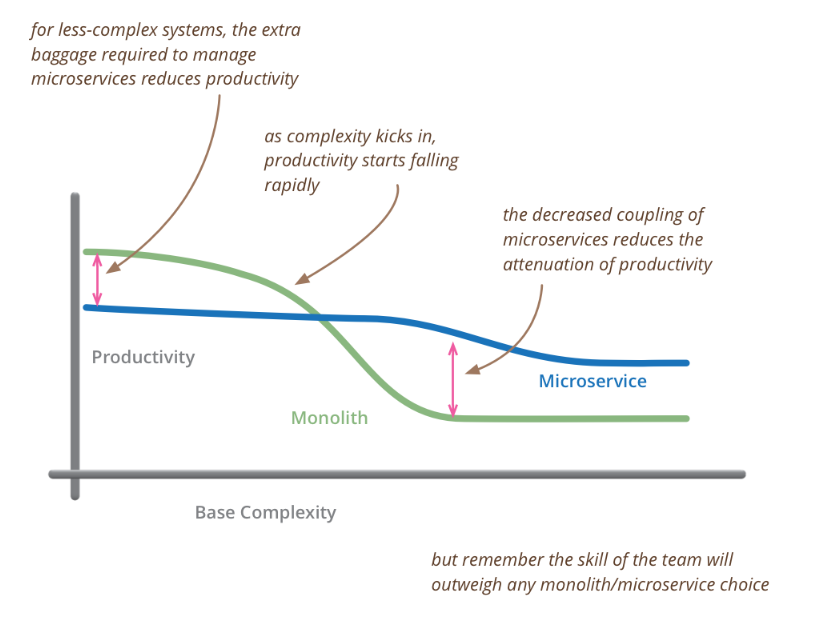
\includegraphics[scale=0.9]{fowler}
	\caption{Complexitatea si productivitatea in arhitecturi diferite}
	\label{fowler}
  	\end{figure}
  	\paragraph{}Un alt exemplu în care microserviciile nu ar fi o soluție bună ar fi aplicațiile care procesează fluxuri de date în timp real, date care vin de la diferiți senzori. Intr-o situație de genul acesta, orice timp contează, iar comunicarea dintre microservicii, chiar dacă este rapidă, poate influența rezultatul, așadar intr-o astfel de situație, o soluție monolit este favorabilă.
  	\paragraph{}În concluzie, am putea spune că stilul arhitectural bazat pe microservicii poate fi aplicat in majoritatea aplicațiilor, dar este indicat să fie folosit doar atunci când aplicația este suficient de mare încât este greu de scalat sau scalarea devine prea scumpă sau în momentul în care sistemul devine atât de complex încât productivitatea este extrem de mică. În capitolul următor va fi prezentată in detaliu o trecere a unei aplicații de la o arhtectură monolitică la una bazată pe microservicii, împreună cu avantajele, costurile si compromisurile care au fost facute, dar si o prezentare a rezultatului final.
  \chapter{Studiu de Caz}
	\section{Introducere}
	\paragraph{}Netflix este o companie care a început prin a vinde sau închiria filme pe DVD-uri. Ulterior furnizând acces online la filme si seriale. Netflix fiind un gigant in industria televiziunii online. Aplicația netflix este o aplicație la scară mondială, care în momentul in care firma a horărat schimbarea arhitecturii avea un trafic de 8 milioane de utilizatori, ajungând la finalul anul 2018 la 139 de milioane de utilizatori.	
	\paragraph{}Dupa cum am discutat până acum, o arhitectură bazată pe microservicii nu are chiar o definiție propriu zisă, dar dupa cum susține Martin Fowler, microserviciile sunt implementarea corectă a arhitecturii bazate pe servicii.
	\paragraph{}În acest capitol vom cuprinde trecerea de la o arhitectură monolit la o arhitectura bazată pe servicii, motivele pentru care s-a facut aceasta tranziție, pașii prin care s-a facut aceasta trecere, avantajele cât si dezavantajele acestei treceri, cât si despre rezultatul final.
	\section{Tranziția către microservicii în compania Netflix}
	\paragraph{}În acest studiu de caz o să ne bazăm pe informațiile oferite de doua dintre personajele importante care au luat parte la tranziția catre microservicii:
	\begin{itemize}
	\item Ruslan Meshemberg
	\item Adrian Cockcroft	
	\item Josh Evans	
	\end{itemize}
	\subsection{Arhitectura aplicației de azi}
	\paragraph{}În următoarea diagrama, este reprezentată, arhitectura bazată pe microservicii a aplicației Netflix.
	\begin{figure}[h]
  	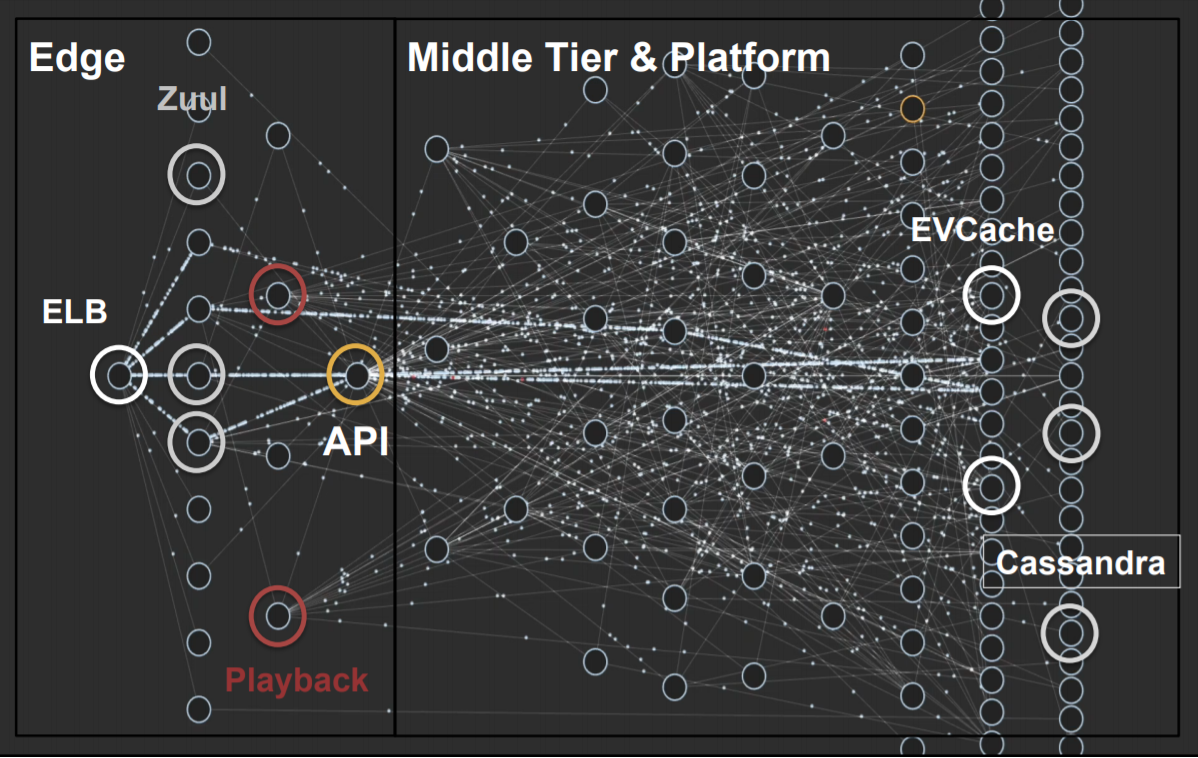
\includegraphics[scale=.651]{netflixarhitecuture}
	\caption{Arhitectura Aplicației Netflix()}  
  	\end{figure}
  	\paragraph{}Făcând o scurtă analiză asupra diagramei, putem să observam că prezentarea este una stratificată, nodul notat „ELB” rebrezintă un balansier de capacitate elastic (Elastic Load Balancer), care se o ocupă cu distrubuirea uniforma a cererilor catre microservicii. Stratul in care avem nodul notat „Zuul”, este un strat de tip proxy care ajută la oprirea atacurilor cibernetice. Iar zona dintre acest strat si „Middle Tier” este reprezentată de componente accesibile clientilor. În partea a 2-a a diagramei, este un strat destul de stratificat de microservicii care conțin mai multa logică si serversc componentelor din prima parte a diagramei. Ultimul strat, cel care contine si nodul notat cu „Cassandra” pe diagramă, reprezintă stratul de acces la bazele de date, datele fiind salvate separat in baza de date NoSQL. Iar intre ultimele 2 straturi   explicate, avem un strat care se ocupa de caching.
  	\paragraph{}O diagramă mai reprezentativă pentru arhitectura bazată pe microservicii a Netflix, care contine mai mult de 500 de microservicii este numita si diagrama de arhitectura „Death Star”(\ref{deathStarArhitecture}).
  	\paragraph{}Așadar, având în vedere scala la care știm deja ca funcționează aplicația Netflix, putem deja considera că arhitectura bazată pe microservicii isi servește bine scopul. În continuare vom discuta efectiv despre motivele, pașii, beneficiile și costurile acestei schimbari de arhitectură.
  	\begin{figure}[h]
  	\centering
  	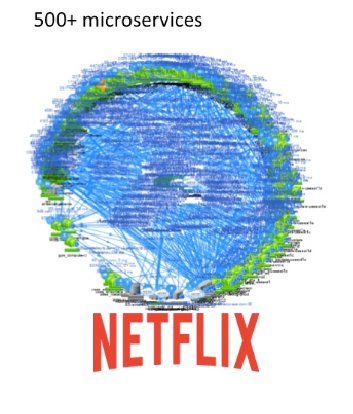
\includegraphics[scale=.8]{deathstararhitecture}
	\caption{Arhitectura Netflix - „Death Star”}  
	\label{deathStarArhitecture}
  	\end{figure}
	\subsection{Motive}
	\paragraph{}Unul dintre primele motive care au înpins compania netflix să iși mute aplicația catre cloud și odata cu asta, inceperea tranziției către noua arhitectură, a fost o criză întampinată în 2008 când baza lor de date a fost coruptă, iar acest lucru a dus la intreruperea activitații timp de 3 zile. 
	\paragraph{}Al doilea motiv a fost ritmul alert în care compania crestea si numarul tot mai mare de utilizatori. Toată lumea era conștientă că numărul de utilizatori va creste si mai mult iar aplicația trebuia scalată din ce in ce mai mult.
	\paragraph{}În momentul în care vorbim de scalabilitate, putem sa ne gândim la asta in 2 feluri, scalare pe veriticala (termenul în engleză „scale up”) sau scalare pe orizontală (termenul în engleză „scale out”). Scalarea pe verticală poate fi văzută ca imbunătățirea constantă a sistemului, nevoia suplimentară de memorie, spatiu pe disk, puterea de procesare mai mare. Acest lucru este posibil doar pană la un anumit punct, ajungându-se la atingearea limitei tehnologice. În plus scalarea pe verticală devenind din ce in ce mai costisitoare.
	\paragraph{}Scalarea pe verticală a devenit în mod rapid, o soluție mult mai ușoară, acest tip de scalare presupune distribuirea aplicației pe mai multe sisteme care lucreaza împreuna. Așadar, în momentul în care aplicația trebuie scalată, este nevoie doar de introducerea unei noi componente in sistem si crearea unei noi instanțe pentru serviciul pentru care se doreste scalarea, iar având in vedere ca Netflix migra in același timp înspre cloud, activarea unei noi unitați si instanțierea unui nou serviciu se poate face foarte simplu și rapid.
	\paragraph{}Mergând mai departe, se dorește eliminarea tuturor punctelor critice, ceea ce înseamnă ca se dorește ca în sistem sa nu existe posibilitatea ca o eroare sa se propage, generând in cascadă și alte erori ale sistemului. Soluția agreeată pentru această problemă a fost crearea de servicii fara stare (în engleză „stateless”), aceestea având proprietatea că anumite date de intrare vor fi procesate si transformate în date de ieșire in același mod indiferent de instanța serviciului. Iar ca si testare a acestei idei, cei de la Netflix folosesc un tool numit „Chaos Monkey”, care aleator distruge cate o instanța al unui serviciu pentru a se garanta că o asemenea eroare nu este propagată în întreg sistemul. Ca acest concept să funcționeze, este nevoie de un balansier, pentru ca datele să fie redistribuite către o altă instanță a aceluiași serviciu.
	\begin{figure}[h]
  	\centering
  	
\includegraphics[scale=.5]{chaos}
	\caption{Chaos Monkey}  
	\label{chaosMonkey}
  	\end{figure}
	\subsection{Avantaje și dezavantaje, costuri și sacrificii}
	\paragraph{}Din punct de vedere al avantajelor pe care microserviciile le aduc, unul dintre ele a fost probabil cel mai apreciat de Netflix, a fost viteza de dezovolare a produsului. Acest lucru, probabil fiind datorat faptului că fiind primul care aduce o imbunătățire sau un lucru nou, este favorizat față de cei care il urmează. Așadar, microserviciile au permis o redistribuire a echipelor, iar noile echipe având responsabilitați separate, conceptul de a astepta dupa o altă echipă pentru a putea sa iti faci treaba, incepe sa dispară.
	\begin{figure}[h]
  	\centering
  	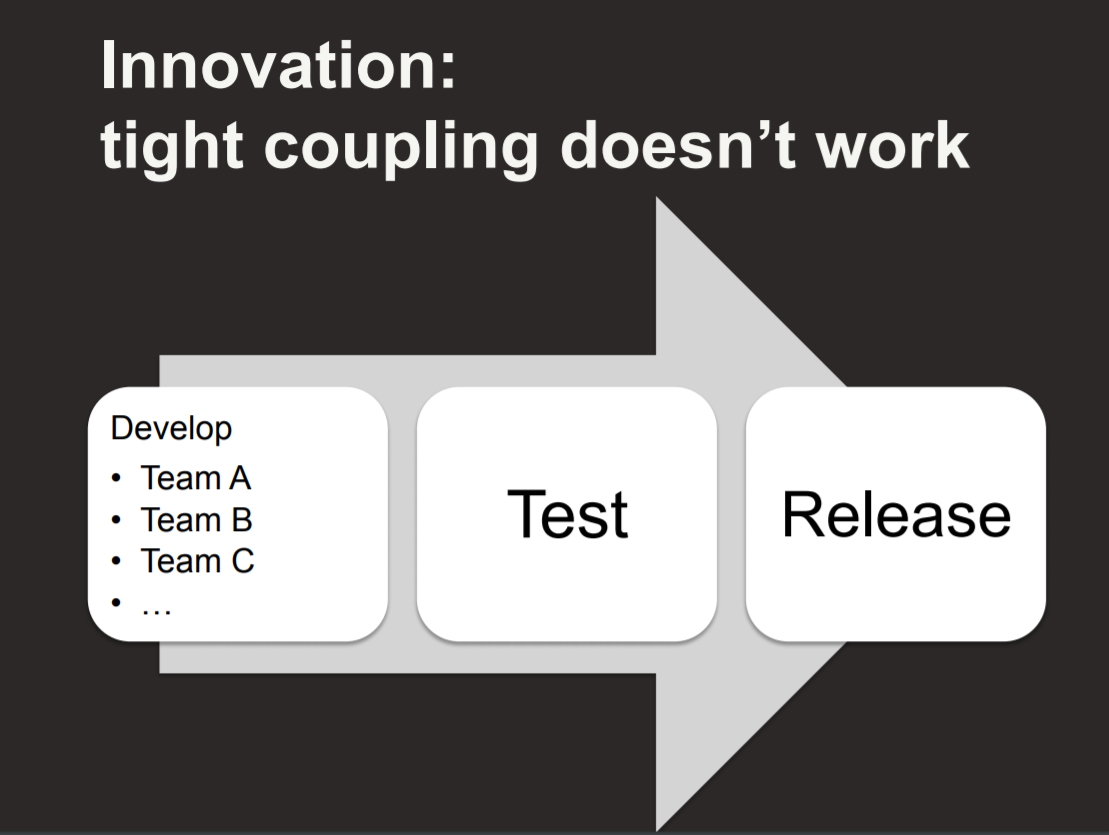
\includegraphics[scale=.4]{tightCoupling}
	\caption{Procesul de dezovoltare intr-o aplicație monolit}  
	\label{tightCoupling}
  	\end{figure}
  	\begin{figure}[h]
  	\centering
  	\includegraphics[scale=.4]{looseCoupling}
	\caption{Procesul de dezovoltare intr-o aplicație bazată pe microservicii}  
	\label{looseCoupling}
  	\end{figure}
  	\paragraph{}După cum se poate observa în prima figură (\ref{tightCoupling}), în prima parte trebuie ca toata aplicația să fie dezvoltată, apoi testată si apoi lansată. Iar în a doua figura (\ref{looseCoupling}), se poate observa ca echipele pot să lucreze fiecare în ritmul lor, nefiind nevoiți să depindă constant de restul. Microserviciile nefiind nevoite să fie lansate in execuție împreună.
	\paragraph{}Pe de altă parte, trebuie să avem in vedere faptul că în această schimbare au fost nevoie și de sacrificii, unele referindu-se la costuri, altele la relație oamenilor din echipe. Printre aceastea se pot numară urmatoarele:
  	\begin{itemize}
  	\item În primul rând, costul de dezvoltare si mentenanță a aplicație a crescut. Motivul fiind următorul: tranziția a fost una de durată, iar in timp ce se crea aplicația cu noua arhitectură, aplicația monolit trebuia sa ramână in picioare. Și pe de alta parte, datele trebuiau sa fie replicate si salvate atat in aplicația noua cât si in cea curentă.
  	\item În al doilea rând, tehnologiile din noua aplicație s-au schimbat partial fața de aplicația monolit, iar compania trebuie sa suporte toate tehnologiile existente din ambele proiecte. Un exemplu este legat de bazele de date, in aplicația monolit existând baze de date relaționale, iar bazele de date din microservicii au devenit baze de date NoSQL. Mai târziu un evoluția noi arhitecturi vor aparea microservicii scrise si in NodeJS, Phyton si alte limbaje de programare.
    \item În al treilea rand, un alt compromis, poate nu atat de mare, a fost în momentul în care compania a ales să traiască intr-o zonă hibridă, asta insemnând ca au inceput sa exite servicii scrise in diferite limbaje de programare cum are fi NodeJS, Phyton si altele. Acest lucru fiind posibil atât timp cât era respectat un format pentru datele de intrare cât și pentru datele ieșire.
  	\item În ultimul rând, un alt compromis care a trebuit făcut a fost schimbarea structurii echipelor. De la echipe specializate pe dezvoltare, echipe specializate pe testare si echipe specializate in lansarea aplicației in mediul online, s-a ajuns la echipe mai mici care să se ocupe de intreg ciclul de viată al unui microserviciu(\ref{endtoend}), De la implementare, pâna la lansarea lui in execuție.
  	\end{itemize}
  	\begin{figure}[h]
  	\centering
  	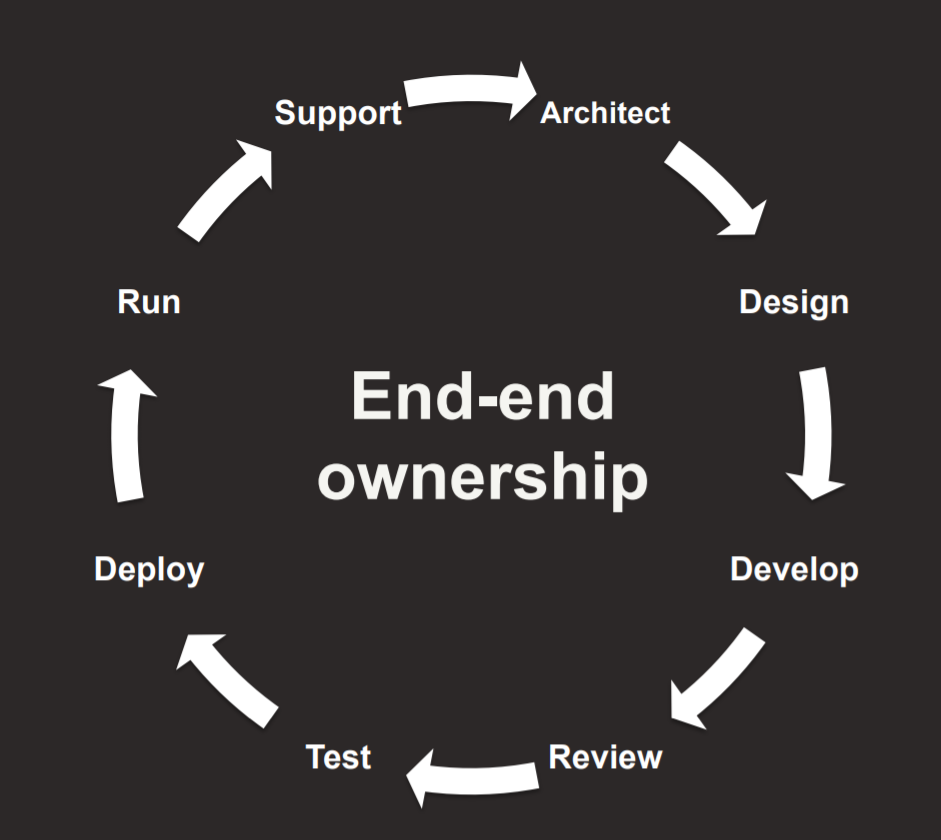
\includegraphics[scale=.7]{endtoend}
	\caption{Ciclul de viață al unui microserviciu}  
	\label{endtoend}
  	\end{figure}
  	\subsection{Descrierea tranziției catre microservicii}
  	\paragraph{}Unul din cei mai importanți oameni care a ajutat la tranziția aplicație catre microservicii si mutarea acesteia in cloud, este specialistul în scalabilitate de la Netflix, Adrian Cockcroft. Dupa cum am amintit și mai sus, posibilitățile de scalare erau pe verticală si pe orizontală. Dupa cum Adrian Cockcroft a susținut in timpul unei conferințe, scalarea pe verticală ar fi însemnat în momentul acela, anul 2009, construirea unui nou centru de date (în engleză „data center”) cu un cost estimativ de aproximativ 100 de milioane de dolari. Iar pe aceași tema, a glumit, spunând ca banii respectivi ar fi mai bine folosiți daca Netflix ar cumpăra inca un sezon din „House Of Cards”(acesta fiind un serial TV). Soluția plauzibilă care a rămas, fiind scalarea pe orizontală.
  	\paragraph{}Primul pas fiind de test, s-a încercat mutarea unui serviciu in cloud, iar alegerea nu a fost intâmplătoare, a fost ales un serviciu care să nu fie in prima linie pentru utilizator, adică un serviciu care mai mult procesează cantităti mari de date in spate. Spre exemplu, algoritmul folosit pentru auto completarea câmpului de cautare. După ce acest pas a fost realizat cu succes, si serviciul era folosit de aplicația monolit, procesul a continuat.
  	\paragraph{}Un alt pas important a fost schimbarea bazei de date, de la baze de date relaționale Oracle, la baza de date NoSQL („Cassandra”). Acesta bază de date este folosită și acum pentru aplicația Netflix. Având în vedere ca este open source(în engleza „open sourse”), Netflix a dezvoltat un feature care ajuta la replicarea usoară a datelor.
  	\paragraph{}După ce întreaga tranziție a fost gata, dupa anul 2012, multe dintre soluțiile aplicate in timpul tranziției au fost publicate, sursele devenind surse deschise.
	\paragraph{}Așadar succesul Netflix se datorează in mare parte lui Adrian Cockcroft, care este un vizionar, reusind tranziția Netflix catre o arhitectura bazată pe microservicii in cloud, intr-un moment in care nimeni nu dorea să creadă ca cloud-ul ar putea să fie o soluție(\ref{toCloud}).
	\begin{figure}[h]
  	\centering
  	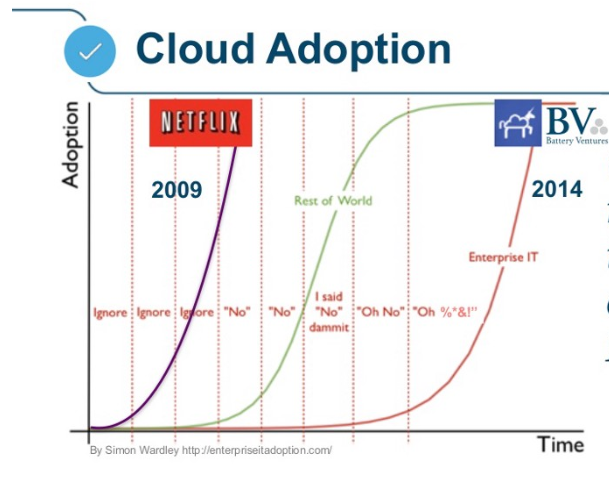
\includegraphics[scale=1]{toCloud}
	\caption{Migrarea catre cloud a aplicațiilor}  
	\label{toCloud}
  	\end{figure}
\chapter{Aplicație Practica}
	\section{Idee}
	\paragraph{}Ideea creării aplicației a venit de la o problemă personală, iar aceasta ar fi următoarea: în fiecare luna scrisorile cu facturi ajung in postă, iar pentru ca nu vin toate in aceeași dată și pentru că nu vin în aceeași data a lunii, trebuie mereu să verifici posta ca să nu uiti sa plătești o facutră. În al doilea rand trebuie sa merg cu facturile la banca ca să le platesc, sau poate chiar firma de la care am primit factura, in caz că nu suporta plata prin bancă. Așadar am decis să creez o aplicație care să ajute în acest scop, iar această aplicație ar putea avea urmatorul enunț.
	\paragraph{}Se dorește construirea unui prototip al unei platforme care să actioneze ca un intermediar între oameni și furnizorii de utilități în care un utilizator să poată sa primească facturile de la toate sau o parte din utilitățile pe care le folosește, sa poată să își încarce o anumită sumă de bani pe platforma (în varianta prototip nu este necesară utilizarea banilor reali), să poată să folosească banii introduși pentru a achita facturile, și să poată vedea detaliile facturilor cât și a tranzacțiilor pe care le efectueză pe platformă. Pentru ca relația dintre utilizatorii normali și furnizori să poată fi creată ușor, conturile utilizatorilor vor folosii CNP-ul pentru a fi create. Din punctul de vedere al furnizorilor de utilități, aceștia pot să fie capabili sa „își conecteze” aplicațiile actuale la platformă, aceasta furnizând puncte de acces pentru adaugarea facturilor, chitanțelor, si pentru cererea unei statistici a tranzactiilor facute catre ei între doua date alese. Toate plățile se vor face pe platformă, acestea efectuându-se fără transfer direct de bani intre platformă si furnizori. Platforma va efectua un singur transfer de bani, la finalul zilei, un singur transfer cu suma totală a platilor efectuate catre furnizorul în cauză. Dupa cum este specificat si mai sus, transferurile nu vor folosii bani reali. Deoarece furnizorii se vor conecta la aplicație prin call-uri la terminalele oferite de aplicație, aceștia vor trimite la fiecare call, un set de date de autentificare generate pentru fiecare furnizor în parte, în momentul în care un furnizor dorește să se lege la platformă. 
	\paragraph{}Având în vedere cerința prezentată, putem deduce că vom avea doua tipuri de utilizatori, utilizatori normali, care vor plăti facturi și furnizorii, care vor adauga facturi, chitanțe și vor genera rapoarte. Putem determina următoarele funcționalități în funcție de tipul utilizatorului:
	\paragraph{}Pentru ultizatorii direcți ai platformei avem următoarele funcționalități:
	\begin{itemize}
	\item Înregistrare
	\item Autentificare
	\item Introducere de bani pe platformă
	\item Vizualizarea facturilor pentru fiecare utilitate
	\item Plata facturilor
	\item Vizualizarea tranzactiilor făcute pe platformă
	\item Vizualizarea chitanțelor.
	\end{itemize}
	\paragraph{}Pentru furnizorii de utilități care doresc conectarea la platformă avem următoarele funcționalități:
	\begin{itemize}
	\item Adăugarea de facturi
	\item Adaugarea chitanțelor după ce o factură a fost plătită
	\item Generarea unui raport cu toate tranzactiile facute intre doua date
	\item Recunoașterea/Autentificarea fiecărui furnizor cu ajutorul unor credențiale alese
	\end{itemize}
	\section{Arhitectura aplicatiei}
	\paragraph{}Aplicația creată are la bază o arhitectură bazată pe microservicii, acest lucru oferind aplicației scalabilitatea necesară, în momentul în care numărul de utilizatori va crește foarte mult, iar acest lucru este datorat de existența unui microserviciu dedicat utilizatorilor. Tot această arhitectură poate oferii flexibilitatea creării unui nou furnizor in sistem, doar prin lansarea unui nou microserviciu cu un fișier de configurarea specific pentru un nou furnizor.
	\begin{figure}[h]
  	\centering
  	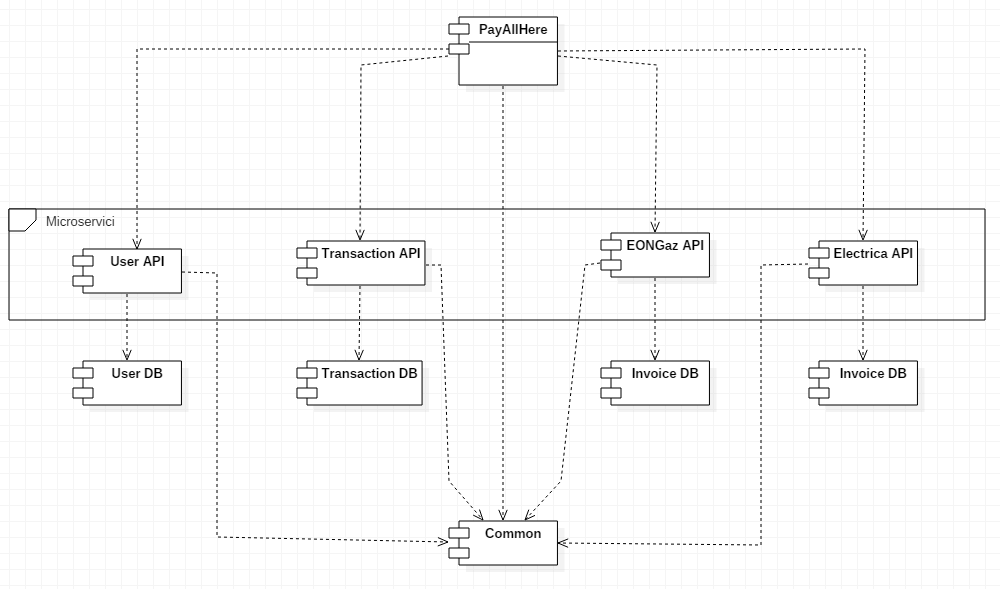
\includegraphics[scale=0.8]{component}
	\caption{Diagrama de arhitectură}  
	\label{component}
  	\end{figure}
  	\paragraph{}În figura de mai jos, figura \ref{component}, se poate observa că aplicația poate fi impărțită din punct de vedere al arhitecturii un in trei straturi și o componentă ajutătatoare denumită „Common”.
	\paragraph{}În stratul superior se poate observa componenta „PayAllHere” care reprezintă de fapt poarta de intrare a unei arhitecturi bazate pe microservicii (în engleza „gateway”). Aceasta este de fapt o aplicație de tip MVC, a cărei singură dependință din proiect este componenta „Common”, dar acest fapt nu crează un cuplaj între componente, deoarece aceasta este doar o librărie (în engleză „Class Library”). Acestă componentă doar cere informații din stratul următor prin call-uri asincrone, ceea ce înseamnă ca există un cuplaj slab intre cele doua straturi.
	\paragraph{}Al doilea strat al aplicației este format din microservicii. Acestea sunt unități independente ale aplicației, nu sunt cuplate între ele, și nu au stare. Fiecare microserviciu se ocupă independent de cate o secțiune a aplicației, în acest fel, avem un microserviciu pentru utilizatori, acesta se ocupă de înregistrarea utilizatorilor, autentificarea lor, cât și să păstreze date despre utilizatori. Un al doilea microserviciu este cel care se ocupă de tranzacții, acesta gestionează tranzactiile care se întamplă pe platformă, cât și de filtrarea unor tranzactii după anumite criterii: data, persone, etc.. 
	\paragraph{}Al treilea și al patrulea microserviciu se ocupă de gestionarea facturilor, fiecare pentru un furnizor specific, ceea ce este bine de precizat, este faptul că structura celor doua microservicii este identică, iar diferențele dintre ele se pot face doar folosindu-se un fișier de configurare, ceea ce înseamnă că adaugarea unui nou furnizor va necesita foarte puțin timp de dezvoltare. Tot procesul fiind doar o lansare in execuție a unui nou microserviciu cu un fișier de configurare schimbat. O prezentare a felului în care un microserviciu de acest tip este implementat se poate observa in diagrama de clase prezentată mai jos, figura \ref{classDiag} 
	\begin{figure}[h]
  	\centering
  	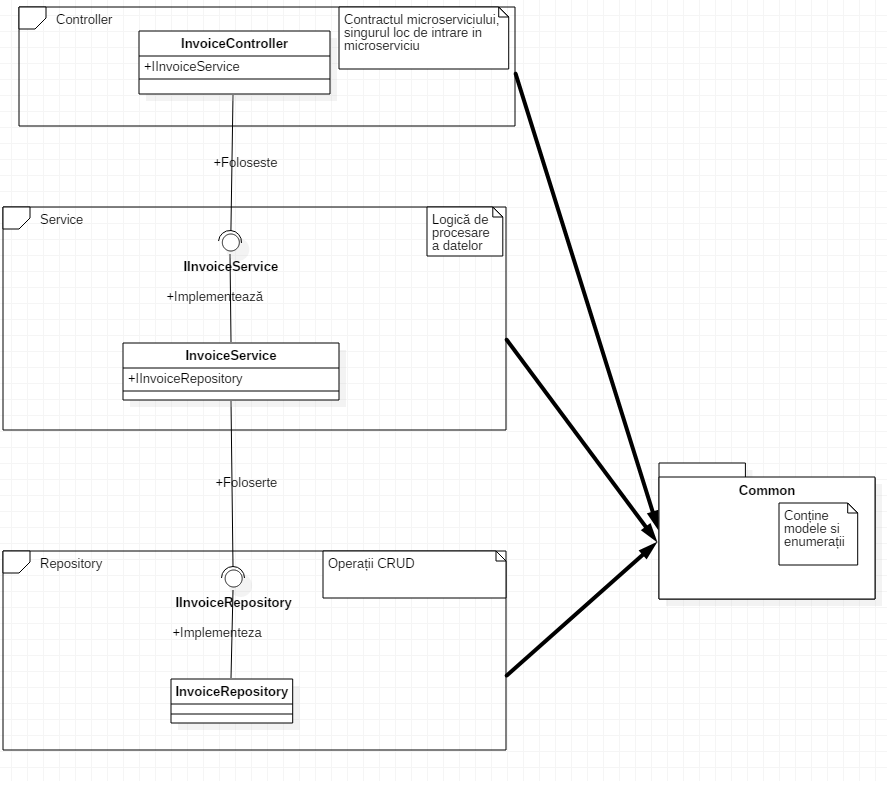
\includegraphics[scale=0.85]{classDiag}
	\caption{Diagrama de clase a unui microserviciu atribuit unui furnizor}  
	\label{classDiag}
  	\end{figure}
  	\paragraph{}Al treilea strat este reprezentat de stratul de persistentă. După cum se poate observa in figura \ref{component}, fiecare microserviciu are cate o bază de date la care are acces unic, ceea ce înseamnă că persistența datelor nu reprezintă un factor de cuplaj între microservicii. 
  	\paragraph{}Ultima componentă este componenta „Common”, in acestă componentă se găsesc modele si enumurații care se folosesc atat in aplicația MVC, cât și în microservicii, acest lucru nu cuplează serviciile, doar se asigură că informația trimisă dintr-o componentă înspre alta să poată sa fie recepționată in același format în care a fost transmisă.
	\section{Persistenta datelor}
	\paragraph{}Dacă e să vorbim de persistența datelor, așa cum s-a menționat mai sus, fiecare microserviciu are acces la propria lui bază de date (\ref{db}).
	\begin{figure}[h]
  	\centering
  	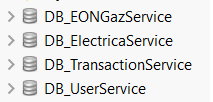
\includegraphics[scale=1]{db}
	\caption{Bazele de date pentru fiecare microserviciu}  
	\label{db}
  	\end{figure}
	\paragraph{}Baza de date folosită este una non realațională, această alegere a fost făcută deoarece este usor de gestionat. În cazul unei modificări in cod asupra clasei salvate in baza de date, schimbarea se va propaga în baza de date făra ca programatorul să depună un efort suplimentar. Fiecare bază de date conține cate o colectie de obiecte (\ref{dbopen}). Așadar, fiindcă baza de date nu este relațională, orice lagatură între doua clase diferite trebuie efectuată la nivel de logică in cod.
	\begin{figure}[h]
  	\centering
  	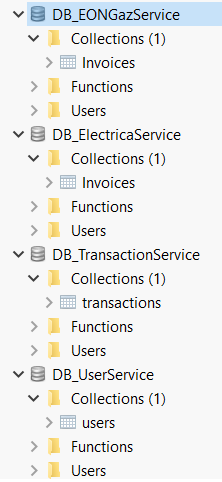
\includegraphics[scale=0.86]{dbopen}
	\caption{Componența bazelor de date}  
	\label{dbopen}
  	\end{figure}
  	\paragraph{}Baza de date folosita este MongoDb. In acestă bază de date se pot salva colectii care au o structura fluidă, dar elementele vor fi salvate in funcție de modelul clasei corespunzătoare. Fiecare obiect este salvat in baza de date serializat JSON. Un exemplu se poate observa mai jos in figura \ref{dbEx}.
  	\begin{figure}[h]
  	\centering
  	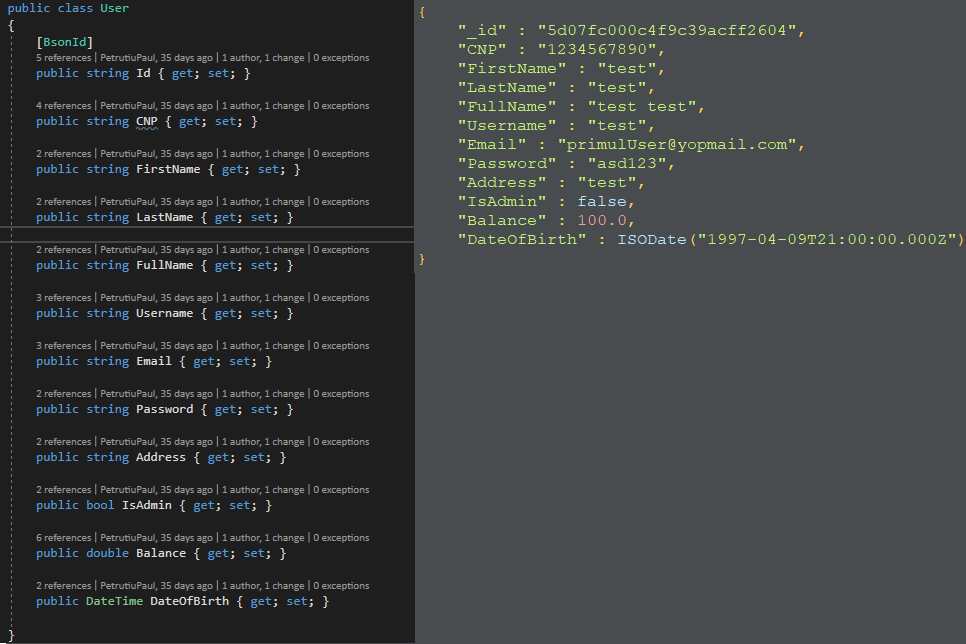
\includegraphics[scale=0.81]{dbEx}
	\caption{Obiect în cod C\# și obiect în baza de date}  
	\label{dbEx}
  	\end{figure}
  	\paragraph{}Singurul lucru care diferă este reprezentare identificatorului unic, care in cod C\# este „Id” iar in baza de date este „\_id”, acest lucru se datorează atributului „[BsonId]” care marchează câmpul „Id” ca fiind identificator unic, iar reprezentarea identificatorului unic in baza de date MongoDb este „\_id” (figura \ref{dbEx}).
	\section{Interacțiunea cu utilizatorul}
	\paragraph{}Din punct de vedere al utilizatorilor, aceștia se împart în doua categorii, utilizatori externi și furnizori de utilitați (gaz, curent, etc.). Iar în funcție de acest criteriu și funcționalitățile pe care deja le-am definit, putem sa considerăm urmatoarele cazuri de utilizare, prezentate în diagrama \ref{usediag}. Este important faputul că doar utilizatorilor externi le este adresată o interfață grafică, furnizorilor ofrindu-li-se acces la anumite puncte de intrare („endpoints”) în aplicație la care se pot conecta cu ajutorul unor apeluri făcute din aplicațiile proprii.
	\begin{figure}[h]
  	\centering
  	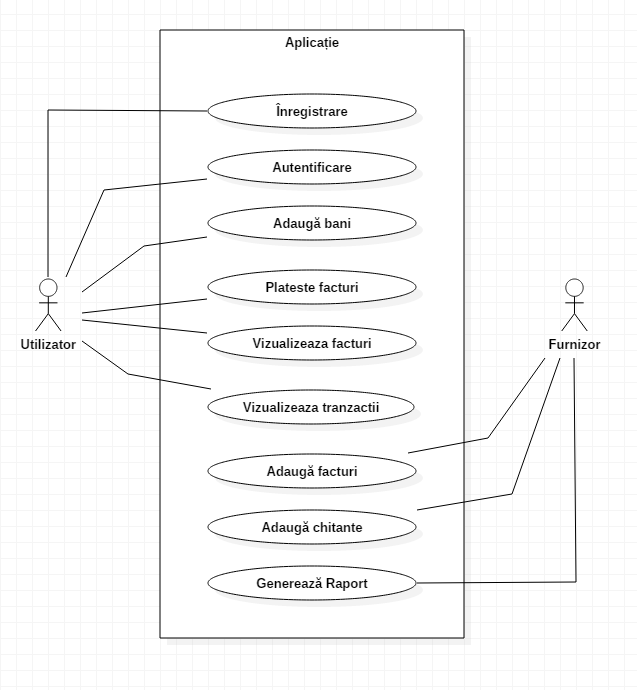
\includegraphics[scale=1]{usediag}
	\caption{Diagrama cazurilor de utilizare}  
	\label{usediag}
  	\end{figure}
  	\paragraph{}În continuare vom exemplifica în detaliu câte un caz de utilizare pentru fiecare dintre tipurile de utilizatori. Pentru utilizatorii externi vom parcurge fiecare pas din fluxul de lucru (în engleză „workflow”) al plății unei facturi, iar pentru utilizatorii de tip furnizor, vom parcurge fiecare pas din fluxul de lucru pentru generarea unui raport pentru doua date selectate. Pentru o mai bună întelegere se va prezenta câte o diagrama de secvența pentru fiecare funcționalitate.
  	\subsection{Plata unei facturi}
  	\paragraph{}Acest caz de utilizare a fost ales deoarece este unul mai complex, acesta implicând aproape toate microserviciile. Pentru completarea cu succes al acestei operații, se vor efectua următoarele evenimente:
  	\begin{itemize}
  	\item Utilizatorul se autentifică
	\item Utilizatorul accesează pagina cu furnizori 	
  	\item Utilizatorul deschide lista de facuturi de la un furnizor (spre exemplu: facutrile de curent)
  	\item Alege factura pe care doreste sa o platească
  	\item Introduce suma pe care doreste să o plătească
  	\item Se actualizează balanța utilizatorului
  	\item Se salvează tranzactia
  	\item Se modifica suma ramasă de plată pentru factura respectivă.
  	\item Utilizatorul este întors pe pagina cu facturi.
  	\end{itemize}
  	\paragraph{}O secvență de plată a unei facturi se consideră un succes în momentul în care se salvează cu succes tranzacția efectuată, iar balanța unui utilizator cat și suma ramasă de plată este actualizată corect.
  	\paragraph{}Unul din motivele pentru care o secvență de plată nu se va executa cu succes poate fi produsă de încercarea plății unei sume care nu este disponibilă în contul curent. În acest caz se va afișa un mesaj corespunzător, iar utilizatorul poate ulterior să încarce o sumă de bani pe platformă iar apoi sa reia procesul de plată a facturii.
  	\paragraph{}După cum se poate observa și în figura \ref{utilizseq}, utilizatorul interacționează cu aplicația MVC, iar aceasta comunică prin apeluri asincrone cu microserviciile care se ocupă de datele utilizatorului, datele despre facturilor furnizorului cât și de tranzacții. Apelurile între microservicii sunt apeluri asincrone de tip HTTP. În diagrama \ref{utilizseq} nu este reprezentat și stratul de persistența, dar putem considera ca fiecare apel la un microserviciu determină o interogare pe baza de date.
  	\begin{figure}[h]
  	\centering
  	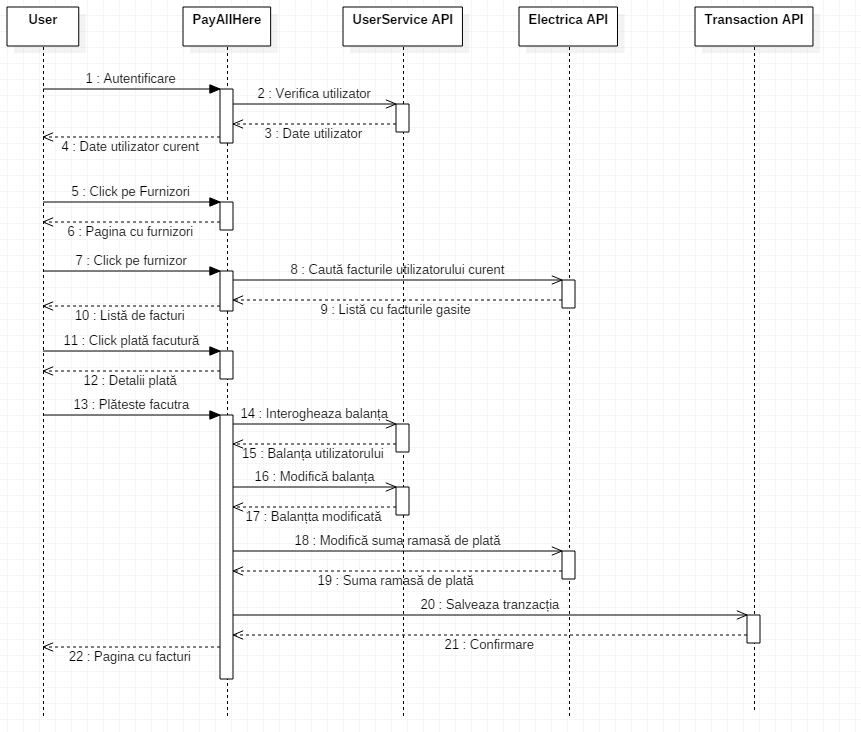
\includegraphics[scale=0.9]{utilizseq}
	\caption{Diagrama de secvență pentru plata unei facturi}  
	\label{utilizseq}
  	\end{figure}
  	\subsection{Generarea unui raport}
  	\section{Analiza arhtecturii}
\chapter{Concluzii}

\bibliographystyle{apacite}
\bibliography{referinte}

\begin{flushleft}
\textbf{Cockcroft, Adrian. 2015. \texttt{Talking microservices with the man who made Netflix’s cloud famous. [interviu cu] Derrick Harris. 2015.}}
\end{flushleft}

\begin{flushleft}
\textbf{
Cockroft, Adrian. 2014. \texttt{Migrating to Microservices by Adrian Cockroft. YouTube. [Interactiv] 2014. https://www.youtube.com/watch?v=1wiMLkXz26M.}}
\end{flushleft}

\begin{flushleft}
\textbf{
Erl, Thomas. 2009. \texttt{SOA Design Patterns. Crawfordville Indiana : Prentice Hall, 2009.}}
\end{flushleft}

\begin{flushleft}
\textbf{
Fowler, Martin. 2014. \texttt{Microservices, 2014,. MartinFowler.com. [Interactiv] 2014. https://martinfowler.com/articles/microservices.html.}}
\end{flushleft}



\end{document}
